\section{Calcium indicators and transgenic lines}
\label{sec:sectionb}

%1. Lin, M. Z. $\&$ Schnitzer, M. J. Genetically encoded indicators of neuronal activity. Nat. Neurosci. 19, 1142–1153 (2016).
%you will use transgenic mice that express GCaMP6 in most neurons of the cortex

In the experimental efforts of this project, there's need for large-scale recordings of neural activity. A myriad of different indicators has been presented in literature and used to divergent extends, being that the suitability of each method to each experimental configuration varies with the priority weights given to factors as the neural events detection fidelity, the specificity of the expressed cell types, and the aimed recording's temporal resolution.

In transgenic mice, given neural processes can be marked and visibly expressed. Genetically encoded indicators of neural activity (GEAIs) are optical indicators that allow for observations that cannot come from electrodes or functional magnetic resonance imaging, accessing neuron's populations' dynamic evolutions over time, within a simultaneous, non-intrusive and less biased observation (for a review, \cite{Lin2016}).

These indicator's have different response curves and response kinetics, and the selection of the appropriate GEAI additionally entails consideration about its responsiveness and reporting speed to given neural events.

A way of accessing the synaptic excitation occurrence is by means of calcium indicators. $Ca^{2+}$ regulates the fusion of synaptic vesicles: Presynaptic terminals contain voltage-gated $Ca^{2+}$ channels (VGCC) in their membranes and their opening occurs when excited by a presynaptic action potential that results in the influx of $Ca^{2+}$ which triggers neurotransmitter release. This influx also happens as action potentials propagate throughout the neuron. In this way, the calcium entry amplifies the marker of neural activity that is wished to detect, by transforming the transient events in the presynaptic membrane into biochemical more prolonged and more widely localized changes.

However, some limitations restrain the use of this sort of indicators: The temporal precision of the process is limited, as the involved half-decay times can be long: In different family's of GECIs, a trade-off emerges between the signal's responsiveness' strength and it's temporal accuracy.

In the current project, a suited GECI was selected from the ultra-sensitive GCaMP6 series \cite{Chen2013}. GCaMP consists of three main components: circularly permuted green fluorescent protein, cpGFP, the chromophore, that is, the region that determines the colour of the compost; calcium-binding protein calmodulin, CaM, and CaM-interacting M13 peptide. Through mutagenesis of this compound, optimizing for sensitivity, GCaMP6 was selected. Besides its great sensitivity, GCaMP6 indicators allow the reliable detection of individual action potentials, the imaging of large neuron populations and small synaptic compartments, all over long time scales. There are GCaMP6 variants suited for different applications, with several overall brightnesses, rise and decay kinetics and calcium affinity properties.

The expression of this compound could be achieved by viral gene transfer using adeno-associated viruses (AAVs). However, besides introducing some level of invasiveness, this method produces different degrees of expression in neurons accourding to their distance to the infection site as well as a continuing increase of expression over time until possible damage to the cells, limiting the imaging time interval of opportunity. These disadvantages can be obviated by transgenic expression of GECIs. The mice that will serve as subjects in this thesis project were genetically modified as to express GCaMP6 in most neurons of the cortex under the Thy1 promoter (\cite{Dana2014}). 

GCaMP6 increases green fluorescence in the presence of calcium (image \ref{GCaMP6Functioning}). As a released neurotransmitter or an action potential opens a VGCC, entering calcium induces the biding of calmodulin (CaM) to a peptide (RS20, homologous to M13). This causes the repositioning of Arg337 (in the CaM domain) which in turn leads to the protonation (loss of a proton) from the chromophore. As the acid dissociation constant decreases, ($pKa= - \log \frac{[A^-][H^+]}{[HA]}$, with $HA$ a generic acid that dissociates into $A^-$) this conformational change of the chromophore induces an absorbance shift and, upon blue excitation, green emission is increased.


\begin{figure}[h]
\center
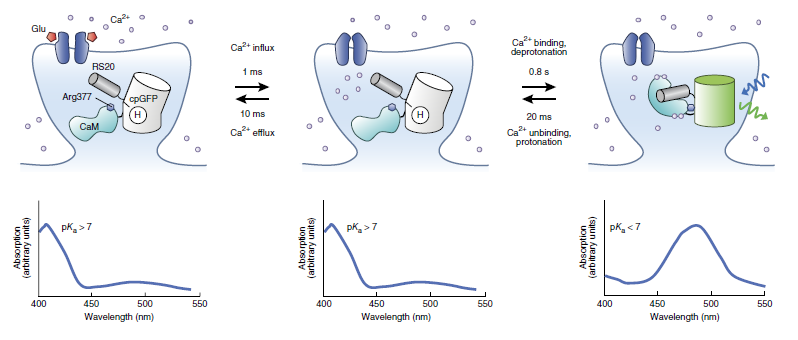
\includegraphics[scale=0.75]{Figures/3.Chapter/GCamp6functioning.png}
\caption{GCaMP6 principle of expression functioning. Process of $Ca^{2+}$ influx, binding, deprotonation and light emission with incread green fluorescence by excitation of blue light (top row) as an absorbance shift with new peak value at ~490 nm is induced by means of chromophore's pH lowering (bottom row).  Image adapted from \cite{Lin2016}.}
\label{GCaMP6Functioning}
\end{figure}

%1. Chen, T.-W. et al. Ultrasensitive fluorescent proteins for imaging neuronal activity. Nature 499, 295–300 (2013).%original GCamp paper

%1. Dana, H. et al. Thy1-GCaMP6 Transgenic Mice for Neuronal Population Imaging In Vivo. PLoS One 9, e108697 (2014). %mice I will use